\section{Combinatoria}
\subsection{Números de Catalán}

Se puede calcular con $C_0 = C_1 = 1$,
$$C_n = \sum_{k = 0}^{n - 1} C_kC_{n - 1 - k} = \frac{1}{n + 1}\binom{2n}{n} = \frac{4n + 2}{n + 2}C_{n - 1},\; n \geq 2.$$
El $n$-ésimo número de Catalán $C_n$ cuenta
\begin{itemize}
    \item La cantidad de secuencias de paréntesis balanceadas de longitud $2n$.
    \item La cantidad de maneras distintas de agrupar $n + 1$ factores con paréntesis.
    \item La cantidad de triangulaciones de un polígono convexo de $n + 2$ lados.
    \item La cantidad de maneras de unir $2n$ puntos en una circunferencia con cuerdas sin que ningún par se corte.
    \item La cantidad de árboles binarios completos con $n$ nodos \textit{internos} no isomorfos. Los nodos \textit{internos} son aquellos con dos hijos.
    \item La cantidad de árboles binarios enraizados completos no isomorfos con $n + 1$ hojas.
    \item La cantidad de árboles enraizados planos no isomorfos con $n + 1$ nodos.
    \item La cantidad de árboles binarios no isomorfos con exactamente $n$ nodos.
    \item La cantidad de caminos monótonos en un tablero de $n \times n$ que van de $(0, 0)$ a $(n, n)$ sin que cruce la diagonal que une $(0, 0)$ con $(n, n)$.
    \item La cantidad de permutaciones de tamaño $n$ que son ordenables con una pila (mientras top() $\leq x$, pop(). Luego push($x$). Al final haz pop() de los elementos restantes de la pila). Equivalentemente la cantidad de permutaciones que no contienen el patrón $231$: no existen índices $i < j < k$ tales que $a_k < a_i < a_j$.
    \item La cantidad de permutaciones de tamaño $n$ que no contienen el patrón $123$: no existen índices $i < j < k$ tales que $a_i < a_j < a_k$.
    \item La cantidad de particiones no cruzadas de un conjunto de tamaño $n$.
    \item La cantidad de maneras de cubrir una escalera con $n$ escalones, con la altura del $i$-ésimo escalón siendo $i$, mediante $n$ rectángulos.
    \item La cantidad de maneras de unir $n$ cuadros de $1 \times 1$ tales que cada cuadro tenga a otro cuadro adyacente a sus lados y, cada columna de cuadros tenga una altura absoluta mayor o igual a la altura absoluta a la columna previa. Cada uno de estos polígonos tiene un perímetro de $2n + 2$.
\end{itemize}

\textbf{Triángulo de Catalán.} Sean $n, k \in \Z_{\geq 0}$, definamos
$$C_{n, k} = \begin{cases}
    0, &n < k \text{ o } n, k < 0,\\
    1, &n = k = 0,\\
    C_{n, k - 1} + C_{n - 1, k}, &k \leq n.
\end{cases}$$

Entonces $C_{n, n} = C_n = \sum_{k = 1}^{n - 1} C_{n - 1, k}$. El número $C_{n, k}$ se puede interpretar como la cantidad de caminos desde $(n, k)$ del Triángulo de Catalán hasta $(0, 0)$. Por lo que tiene sentido que $C_{n, n} = C_n$, dado que $C_{n, n}$ es la cantidad de caminos monótonos desde $(n, n)$ a $(0, 0)$ en un tablero de $n \times n$ que no cruzan la diagonal que une $(0, 0)$ y $(n, n)$.
\begin{figure}[H]
    \centering
    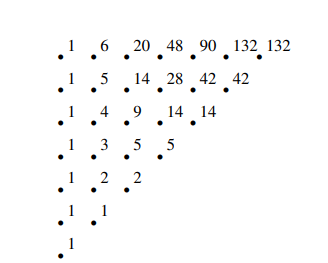
\includegraphics[width=0.5\linewidth]{img/triangulo_catalan.png}
    \caption{Triángulo de Catalán hasta $n = 6$.}
\end{figure}

\subsection{Números de Narayana}

Sean $n, k \in \Z^+$ con $k \leq n$, los números de Narayana se definen como
$$N(n, k) = \frac{1}{n}\binom{n}{k}\binom{n}{k - 1}.$$

Se cumple que
$$N(n, k) = N(n, n - k + 1),$$
$$\sum_{k = 1}^n N(n, k) = C_n,$$

donde $C_n$ es el $n$-ésimo número de Catalán. El número $N(n, k)$ cuenta

\begin{itemize}
    \item La cantidad de secuencias de paréntesis balanceadas con $2n$ paréntesis y $k$ distintos anidamientos, es decir, $k$ ocurrencias de la subcadena $()$.
    \item La cantidad de caminos distintos desde $(0, 0)$ a $(2n, 0)$ dando pasos hacia arriba o abajo y siempre avanzando una unidad en cada paso (diagonales), de manera que haya exactamente $k$ picos. Equivalentemente a la cantidad de maneras de ordenar $n$ $1$'s y $n$ $(-1)$'s en una secuencia $a_i$ tales que si $S_i$ es la suma parcial de $a_i$, entonces $\set{S_i}$ tiene exactamente $k$ máximos locales.
    \begin{figure}[H]
        \centering
        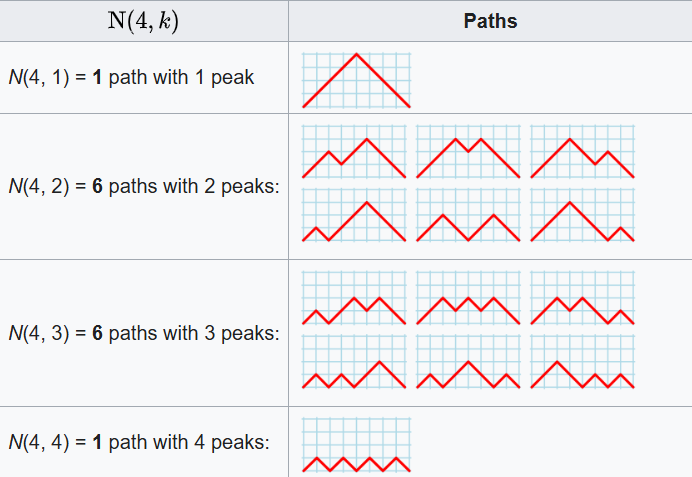
\includegraphics[width=0.5\linewidth]{img/caminos_picos_narayana.png}
        \caption{Caminos de $(0,0)$ a $(8, 0)$ que cuenta $N(4, k)$.}
    \end{figure}
    \item La cantidad de árboles enraizados con $n + 1$ nodos y $k$ hojas.
    \item La cantidad de particiones no cruzadas de un conjunto de tamaño $n$ en exactamente $k$ subconjuntos.
\end{itemize}


\subsection{Particiones Enteras}
Genera todas las particiones de un número \(n\) como suma de enteros positivos en orden no creciente. Complejidad: Tiempo \(O\Pa{ \frac{13^{\sqrt{n}}}{n} }\) – Memoria extra \(O(n)\).

\begin{minted}{cpp}
void generar(int n, int maximo, vi &actual){
    if(n == 0){// Aqui trabajar con actual
        return; }
    for(int i = min(n, maximo); i >= 1; --i){
        actual.pb(i);
        generar(n - i, i, actual);
        actual.pop_back();
    }
}
\end{minted}
La función de partición \( p(n) \), que cuenta el número de formas distintas de escribir \( n \) como suma de enteros positivos sin importar el orden,

% INSERTAR TABLA
\begin{table}[H]
	\centering
	\begin{tabular}{|c|cccccccc|}
		\hline
		$n$ & 1 & 2 & 3 & 4 & 5 & 6 & 7 & 8\\
		\hline
		$p(n)$ & 1 & 2 & 3 & 5 & 7 & 11 & 15 & 22\\
		\hline
		\hline
		$n$ & 9 & 10 & 11 & 12 & 13 & 14 & 15 & 16 \\
		\hline
		 $p(n)$ & 30 & 42 & 56 & 77 & 101 & 135 & 176 & 231\\
		\hline
	\end{tabular}
	\caption{Particiones enteras}
\end{table}

Tiene la siguiente aproximación asintótica para valores grandes de $n$, conocida como la fórmula de Hardy-Ramanujan:

\[
p(n) \sim \frac{1}{4n\sqrt{3}} \exp\left( \pi \sqrt{\frac{2n}{3}} \right)
\]